\chap{Ein Roboterhaustier}
\label{ch.pet}

In diesem Kapitel machen wir den Thymio zu einem \emph{autonomen Roboter}.
Wir programmieren ihn so, dass er unabhängige Verhalten hat, wie dies normalerweise mit
Katzen oder Hunde in Verbindung gebracht wird. Diese Verhalten können wir mittels \textit{Rückkkoppelung}
erreichen: Der Roboter nimmt ein Ereignis in der Umwelt mit seinen Sensoren
wahr und verändert seine Aktionen entsprechend.

\sect{Der Roboter gehorcht dir}

Zuerst lehren wir den Roboter, uns zu gehorchen. 
Und zwar so, dass er sich normalerweise nicht bewegt; 
wenn er aber deine Hand vor sich wahrnimmt, soll er
zu deiner Hand fahren.

Der Roboter hat vorne fünf horizontale Distanzsensoren und zwei hinten.
Diese sind ähnlich aufgebaut, wie die Bodensensoren auf der Unterseite des Roboter, die wir in \cref{c.moving} benutzt haben. Führe deine Hand langsam näher an
die Sensoren des Roboters. Wenn deine Hand nahe genug ist, leuchtet ein kleines, rotes
Licht neben dem Sensor auf und zeigt so an, dass die Hand erkannt wurde (\cref{fig.detect}).


\begin{figure}
\begin{center}
\gr{detect}{.6}
\caption{Die Vorderseite des Thymio. Zwei Distanzsensoren haben die Finger
erkannt.}
\label{fig.detect}
\end{center}
\end{figure}

Der Block \blksm{event-prox} wird gebraucht, 
um zu erfahren, ob etwas nahe am Sensor ist oder nicht. 
Beide Fälle werden als Ereignis gewertet. 
Die schmalen, grauen Quadrate (fünf vorne und zwei hinten) können wahrnehmen,
 wann ein Ereignis stattfindet. 
Indem auf ein Quadrat gedrückt wird, 
ändert sich dieses von grau auf weiss, 
von weiss auf rot und zurück auf grau.
Die Beduetung der Farben ist für diesen Block:

\begin{itemize}
\item \textbf{Grau}: Der Sensor beeinflusst das Programm nicht.
\item \textbf{Rot}: Eine Aktion wird ausgelöst, falls ein Objekt im Bereich des Sensors angegeben wird.
\item \textbf{Weiss}: Eine Aktion wird gestartet, falls \emph{kein} Objekt im Bereich des Sensors angegeben wird.
\end{itemize}

%\importantbox[Boden- und horizontale Sensoren]{
\importantbox{
Achte darauf, das Verhalten der horizontalen Sensoren nicht mit dem Verhalten der Bodensensoren zu verwechseln.
\begin{itemize}[noitemsep,nosep,leftmargin=*]
\item Bei den horizontalen Sensoren bedeutet ein weisses Quadrat, dass ein Ereignis stattfindet, wenn \emph{nichts in der Nähe} ist. Während ein rotes Quadrat bedeutet, dass ein Ereignis stattfindet, wenn \emph{etwas in der Nähe} ist.
\item Bei den Bodensensoren bedeutet ein weisses Quadrat, dass ein Ereignis stattfindet, wenn \emph{nur wenig Licht reflektiert wird}. Während ein rotes Quadrat bedeutet, dass ein Ereignis statfindet, wenn \emph{viel Licht reflektiert wird}.
\end{itemize}
Das physikalische Prinzip dieser beiden Typen von Sensoren ist ähnlich. Wegen deren verschiedener Platzierung ist ihr Verhalten jedoch verschieden.
}

Damit  ein bestimmtes Verhalten des Roboters ausgelöst wird, 
brauchen wir die beiden Ereignis-Aktions Paare, 
wie in der Abbildung~\ref{fig.follow-hand} gezeigt. 
Das erste Paar besteht aus dem zentralen vorderen Sensor mit der Einstellung weiss. 
Die dazugehörige Aktion ist, dass die Motoren ausgeschaltet werden. 
Somit wird der Roboter stehen bleiben, falls er schon still gestanden ist oder anhalten, 
falls er in Bewegung war. 
Das zweite Paar besteht aus dem zentralen vorderen Sensor mit der Einstellung rot. 
Die dazugehörige Aktion ist, dass beide Motoren schnell laufen, indem die Quadrate der Schieberegler ganz nach oben geschoben werden. 
Falls du nun deine Hand vor den Roboter hältst, wird eine Aktion ausgelöst, die bewirkt, 
dass beiden Motoren rasch vorwärtsdrehen und  der Roboter sich vorwärts auf die Hand zubewegt.


\begin{figure}
\begin{floatrow}
	\ffigbox
	{\caption{Bewegung zu der Hand hin}\label{fig.follow-hand}}
	{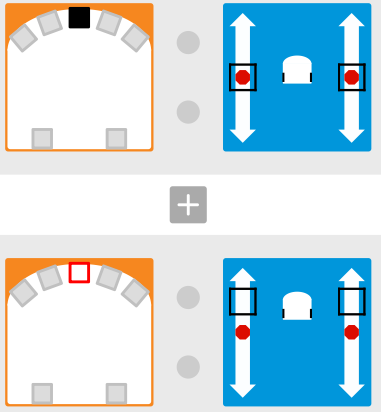
\includegraphics[width=.4\textwidth]{likes-forward}}
	\ffigbox
	{\caption{Ein Bulldozer mit Raupenantrieb}\label{fig.bull}}
	{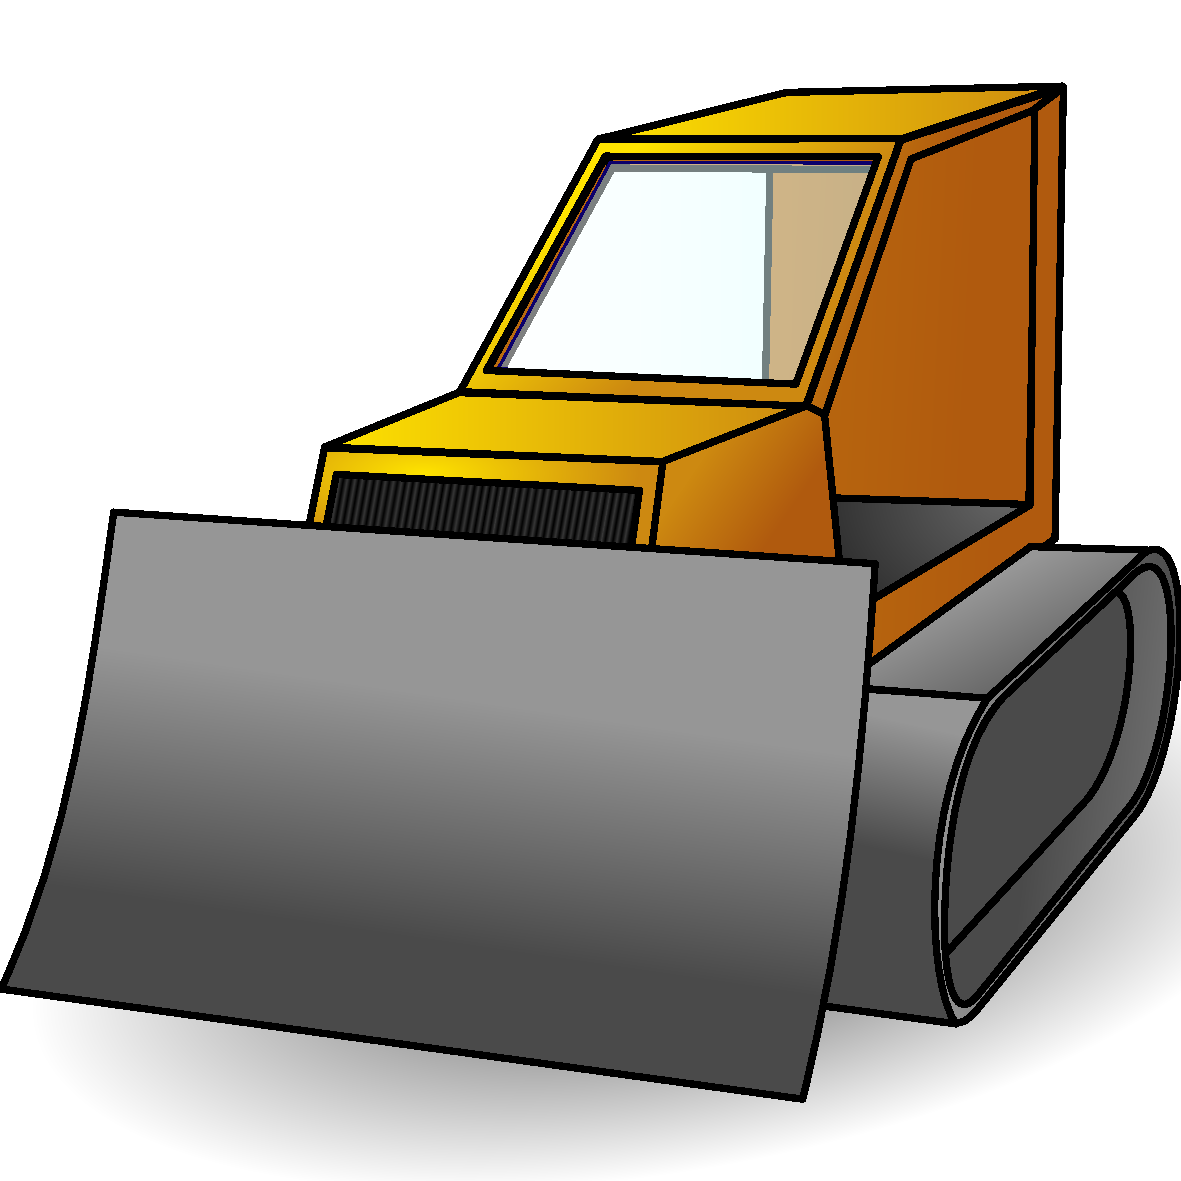
\includegraphics[width=.35\textwidth]{bulldozer}}
\end{floatrow}
\end{figure}

\sect{Steuere den Thymio Roboter}

Der Thymio Roboter hat kein Steuerrad wie ein Auto oder einen Lenker wie ein Fahrrad.
Wie kann der Roboter nun gelenkt werden? Der Roboter benutzt ein \emph{Differentialgetriebe},
welches ähnlich funktioniert wie bei Raupenfahrzeugen, z.B. einem Bulldozer (Figure~\ref{fig.bull}).
Die gewünschte Richtung wird anstelle eines Steuerrads mit \emph{unterschiedlichen} Geschwindigkeiten
des linken und des rechten Rades erreicht. Dreht das rechte Rad schneller als das linke,
biegt das Fahrzeug nach links ab und dreht das linke Rad schneller als das rechte, biegt das Fahrzeug rechts ab.


In VPL kannst du das Differentialgetriebe anwenden, indem du den linken und rechten Schieberegler des Motoraktionsblock einzeln einstellst und dadurch die Geschweindigkeit der Räder verschieden einstellen kannst.
Je grösser der Unterschied der Geschwindigkeiten,
desto enger wird die Kurve. Indem die Räder in unterschiedliche Richtungen drehen,
wird ein möglichst grosser Unterschied der Geschwindigkeiten erreicht. 
Tatsächlich dreht sich das Fahrzeug auf der Stelle, 
falls sich die Räder mit der genau \emph{gleichen} 
Geschwindigkeit in entgegengesetzter Richtung bewegen.

Zum Beispiel wird im Aktionsblock \blksm{differential} der linke Regler auf schnelle Geschwindigkeit rückwärts 
und der rechte Regler auf schnelle Geschwindigkeit vorwärts eingestellt. 
Als Resultat wird der Roboter eine enge Linkskurve vollführen, 
wie dies auf dem kleinen Bild des Roboter bzw. des Motoraktionsblocks dargestellt ist.

Experimentiere mit dem Ereignis-Aktions Paar \blkc{turning}.

Stelle den linken und den rechten Regler ein.
Lass das Programm laufen und drücke den zentralen Schalter.
Um den Roboter zu stoppen, klicke auf \blksm{stop}.
Nun kannst Du die Regler ändern und es erneut ausprobieren.

\trickbox{Das Icon des Thymio in der Mitte des Motoraktionsblock zeigt eine Animation der Bewegung des Roboters, wenn du die Regler einstellst.
}

\sect{Der Roboter mag dich}

Ein echtes Haustier folgt dir manchmal.
Damit der Roboter deiner Hand folgt,
musst du zwei weitere Ereignis-Aktions Paare hinzufügen.
Falls der Roboter ein Objekt vor seinem
ganz links platzierten Distanzsensor wahrnimmt,
soll er nach links und falls er ein Objekt
vor seinem ganz rechts platzierten Distanzsensor wahrnimmt, soll er nach rechts abbiegen.

{\raggedleft \hfill Program file \bu{likes.aesl}}

Das Programm für "der Roboter mag dich"  besteht aus zwei Ereignis-Aktions Paaren
(Figure~\cref{fig.likes}).
Probiere die Regler an jedem Motoraktionsblock aus!

\begin{figure}
	\subfigure[Der Roboter mag dich]{
		\label{fig.likes}
		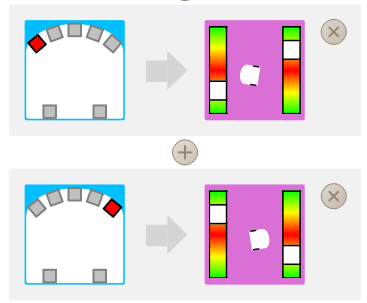
\includegraphics[width=.4\textwidth]{likes-turns}
	}
	\hfill
	\subfigure[Der Roboter mag dich nicht]{
		\label{fig.hates}
		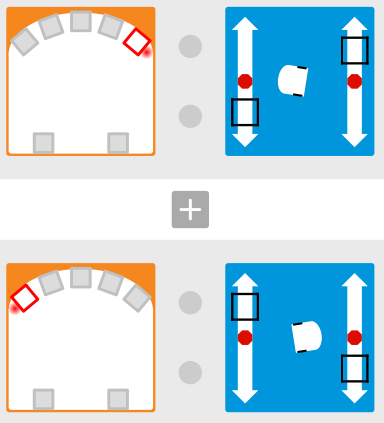
\includegraphics[width=.4\textwidth]{hates}
	}
	\caption{Programm für das Roboterhaustier}
\end{figure}

\exercisebox{\thechapter.1}{
Modifiziere den Haustierroboter so,
dass er vorwärts fährt, falls das Programm am laufen ist
und dass er stoppt, falls er das Ende des Tisches (oder ein Klebeband) wahrnimmt.}

Wie in \cref{c.moving} erklärt, wird von einer weissen Oberfläche viel Licht reflektiert, währen von einer schwarzen Oberfläche wenig Licht reflektiert wird. Je nach Boden oder Tisch musst du entscheiden,
wann du auf das weisse oder das rote Quadrat drückst,
abhängig vom Boden oder Tisch auf den du den Roboter setztst.


\exercisebox{\thechapter.2}{
Was passiert, falls Du die Reihenfolge des Ereignis-Aktions Paares änderst, 
welches Du in der vorangegangenen Übung verwendet hast?
}

\newpage

\sect{Der Roboter mag dich nicht}

Manchmal mag dein Roboterhaustier in schlechter Laune sein und von deiner Hand zurückweichen. Erstelle ein Programm, welches dieses Verhalten auslöst.

{\raggedleft \hfill Program file \bu{does-not-like.aesl}}

Öffne das Programm für den Haustierroboter, 
der Dich mag und ändere die Zusammenhänge für die Ereignisse mit den Aktionen. 
Das Erkennen eines Hindernisses beim linken Sensor bewirkt, 
dass der Roboter nach rechts abbiegt, 
während das Erkennen eines Hindernisses beim rechten Sensor bewirkt, 
dass der Roboter nach links abbiegt (Figure~\ref{fig.hates}).


\exercisebox{\thechapter.3}{
Experimentiere mit der Auswahl der Sensoren.
Die horizontalen Sensoren werden vorne von links nach rechts wie folgt nummeriert 0,1, 2, 3, 4. Die hinteren Sensoren sind Sensor Nummer 5 auf der linken und Sensor Nummer 6 auf der rechten Seite. Verwende andere Sensoren anstelle von den Sensoren 0 und 4. 
\begin{itemize}[noitemsep,nosep,leftmargin=*]
\item Benutze Sensor 1 bzw. Sensor 3, um den Roboter nach links bzw. nach rechts abbiegen zu lassen.
\item Benutze die Sensoren 0 und 1 bzw. 3 und 4, um den Roboter nach links bzw. nach rechts abbiegen zu lassen.
\item Füge Ereignis-Aktions Paare für die hinteren Sensoren 5 und 6 hinzu.
\end{itemize}
}

\sect{Stelle die Regler genau ein (fortgeschritten)}

Es ist schwierig die Regler so präzise einzustellen, dass die Motoren z.B. mit exakt derselben Geschwindigkeit laufen. Indem die Übersetzung der Ereignis-Aktions Paare im Texteditor betrachtet werden, kann die Genauigkeit erhöht werden. \Cref{fig.textcode} zeigt das Programm, welches bewirkt, dass der Haustierroboter dich mag und dir folgt mit der Übersetzung als Text auf der rechten Seite des VPL Fensters.
Der Text wird automatisch angepasst, wenn du Ereignis-Aktionspaare veränderst.

\begin{figure}
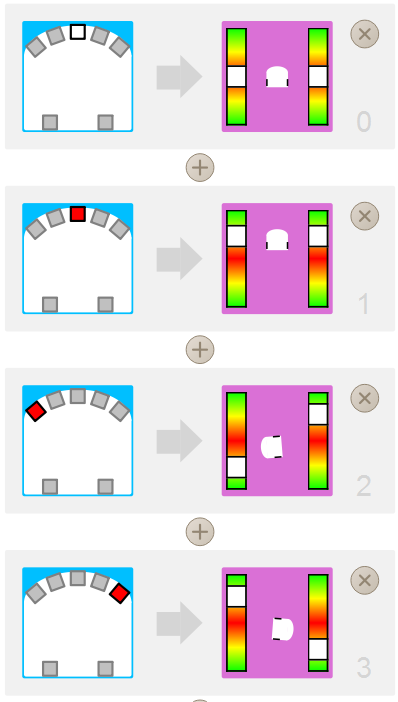
\includegraphics[width=0.3\textwidth]{follow4}
\hfill
\begin{minipage}[b]{0.6\textwidth}
\footnotesize
\begin{lstlisting}
onevent prox
  if prox.horizontal[2] < 400 then
    motor.left.target = 0
    motor.right.target = 0
  end
  if prox.horizontal[2] > 500 then
    motor.left.target = 300
    motor.right.target = 300
  end
  if prox.horizontal[0] > 500 then
    motor.left.target = -300
    motor.right.target = 300
  end
  if prox.horizontal[4] > 500 then
    motor.left.target = 300
    motor.right.target = -300
  end
\end{lstlisting}
\end{minipage}
\caption{A VPL program and the corresponding text program.}
\label{fig.textcode}
\end{figure}

Die Zeile \p{onevent prox} bedeutet:
Immer wenn das Ereignis "Messen der horizontalen Distanz"  des Distanzsensors (\emph{Näherungs}sensor: englisch proximity sensor, abgekürzt \emph{prox}) 
stattfindet (dies findet 10 mal pro Sekunde statt), wird
die folgenden Zeilen des Programms ausgeführt:

Wenn das Ereignis stattfindet, vergleicht Thymio die Sensorenwerte mit der Bedingung
\p{if} \ldots \ \p{then} \ldots \ \p{end}.
Er startet mit dem Testen von Sensor 2 (vorne in der Mitte), wie wir in \p{prox.horizontal[2]} erkennen können.
Falls dieser Wert geringer als 400 ist, stellt Thymio die Geschwindigkeit des linken und rechten Motors auf 0, siehe Zeile \p{motor.left.target = 0} und \p{motor.right.target = 0}.

Jede Zeile
\p{if} \ldots \ \p{then} \ldots \ \p{end} 
testet einen spezifischen Sensor und führt die verbundene Aktion aus oder nicht aus, je nach Resultat des Testes.
Daher ist es mit einem Ereignis-Aktionspaar verbunden:

\begin{enumerate}[start=0,noitemsep,nosep]
	\item Test, ob nichts in der Mitte ist. Ist das wahr, stoppt Thymio.
	\item Test, ob etwas in der Mitte ist. Ist das wahr, fährt Thymio vorwärts.
	\item Test, ob etwas links von der Mitte ist. Ist das wahr, fährt Thymio nach links.
	\item Test, ob etwas rechts von der Mitte ist. Ist das wahr, fährt Thymio nach rechts. 
\end{enumerate}

Hat Thymio schlussendlich alle diese Sensoren ausgewertet, wartet er auf das nächste Ereignis \p{prox} und startet diese Tests von neuem undendlich oft.

Benütze die AsebaStudio Umgebung(\cref{ch.next}), um Programme im Textmodus zu schreiben.


\trickbox{Wenn du die Regler der Motorenaktionsblöcke bewegst, siehst du, dass du die Endgeschwindigkeit der Motoren (\p{moter.X.target}) in 50iger Schritten von $-$500
bis 500 verändert kannst. Indem du die Regler vorsichtig bewegst, kannst Du die Geschwindigkeit auf jeden dieser Werte einstellen.
}